\PassOptionsToPackage{unicode=true}{hyperref} % options for packages loaded elsewhere
\PassOptionsToPackage{hyphens}{url}
\PassOptionsToPackage{dvipsnames,svgnames*,x11names*}{xcolor}
%
\documentclass[]{article}
\usepackage{lmodern}
\usepackage{amssymb,amsmath}
\usepackage{ifxetex,ifluatex}
\usepackage{fixltx2e} % provides \textsubscript
\ifnum 0\ifxetex 1\fi\ifluatex 1\fi=0 % if pdftex
  \usepackage[T1]{fontenc}
  \usepackage[utf8]{inputenc}
  \usepackage{textcomp} % provides euro and other symbols
\else % if luatex or xelatex
  \usepackage{unicode-math}
  \defaultfontfeatures{Ligatures=TeX,Scale=MatchLowercase}
\fi
% use upquote if available, for straight quotes in verbatim environments
\IfFileExists{upquote.sty}{\usepackage{upquote}}{}
% use microtype if available
\IfFileExists{microtype.sty}{%
\usepackage[]{microtype}
\UseMicrotypeSet[protrusion]{basicmath} % disable protrusion for tt fonts
}{}
\IfFileExists{parskip.sty}{%
\usepackage{parskip}
}{% else
\setlength{\parindent}{0pt}
\setlength{\parskip}{6pt plus 2pt minus 1pt}
}
\usepackage{xcolor}
\usepackage{hyperref}
\hypersetup{
            pdftitle={Module 11: Solutions to Recommended Exercises},
            pdfauthor={Emma Skarstein, Michail Spitieris, Stefanie Muff; Department of Mathematical Sciences, NTNU},
            colorlinks=true,
            linkcolor=Maroon,
            filecolor=Maroon,
            citecolor=Blue,
            urlcolor=blue,
            breaklinks=true}
\urlstyle{same}  % don't use monospace font for urls
\usepackage[margin=1in]{geometry}
\usepackage{color}
\usepackage{fancyvrb}
\newcommand{\VerbBar}{|}
\newcommand{\VERB}{\Verb[commandchars=\\\{\}]}
\DefineVerbatimEnvironment{Highlighting}{Verbatim}{commandchars=\\\{\}}
% Add ',fontsize=\small' for more characters per line
\usepackage{framed}
\definecolor{shadecolor}{RGB}{248,248,248}
\newenvironment{Shaded}{\begin{snugshade}}{\end{snugshade}}
\newcommand{\AlertTok}[1]{\textcolor[rgb]{0.94,0.16,0.16}{#1}}
\newcommand{\AnnotationTok}[1]{\textcolor[rgb]{0.56,0.35,0.01}{\textbf{\textit{#1}}}}
\newcommand{\AttributeTok}[1]{\textcolor[rgb]{0.77,0.63,0.00}{#1}}
\newcommand{\BaseNTok}[1]{\textcolor[rgb]{0.00,0.00,0.81}{#1}}
\newcommand{\BuiltInTok}[1]{#1}
\newcommand{\CharTok}[1]{\textcolor[rgb]{0.31,0.60,0.02}{#1}}
\newcommand{\CommentTok}[1]{\textcolor[rgb]{0.56,0.35,0.01}{\textit{#1}}}
\newcommand{\CommentVarTok}[1]{\textcolor[rgb]{0.56,0.35,0.01}{\textbf{\textit{#1}}}}
\newcommand{\ConstantTok}[1]{\textcolor[rgb]{0.00,0.00,0.00}{#1}}
\newcommand{\ControlFlowTok}[1]{\textcolor[rgb]{0.13,0.29,0.53}{\textbf{#1}}}
\newcommand{\DataTypeTok}[1]{\textcolor[rgb]{0.13,0.29,0.53}{#1}}
\newcommand{\DecValTok}[1]{\textcolor[rgb]{0.00,0.00,0.81}{#1}}
\newcommand{\DocumentationTok}[1]{\textcolor[rgb]{0.56,0.35,0.01}{\textbf{\textit{#1}}}}
\newcommand{\ErrorTok}[1]{\textcolor[rgb]{0.64,0.00,0.00}{\textbf{#1}}}
\newcommand{\ExtensionTok}[1]{#1}
\newcommand{\FloatTok}[1]{\textcolor[rgb]{0.00,0.00,0.81}{#1}}
\newcommand{\FunctionTok}[1]{\textcolor[rgb]{0.00,0.00,0.00}{#1}}
\newcommand{\ImportTok}[1]{#1}
\newcommand{\InformationTok}[1]{\textcolor[rgb]{0.56,0.35,0.01}{\textbf{\textit{#1}}}}
\newcommand{\KeywordTok}[1]{\textcolor[rgb]{0.13,0.29,0.53}{\textbf{#1}}}
\newcommand{\NormalTok}[1]{#1}
\newcommand{\OperatorTok}[1]{\textcolor[rgb]{0.81,0.36,0.00}{\textbf{#1}}}
\newcommand{\OtherTok}[1]{\textcolor[rgb]{0.56,0.35,0.01}{#1}}
\newcommand{\PreprocessorTok}[1]{\textcolor[rgb]{0.56,0.35,0.01}{\textit{#1}}}
\newcommand{\RegionMarkerTok}[1]{#1}
\newcommand{\SpecialCharTok}[1]{\textcolor[rgb]{0.00,0.00,0.00}{#1}}
\newcommand{\SpecialStringTok}[1]{\textcolor[rgb]{0.31,0.60,0.02}{#1}}
\newcommand{\StringTok}[1]{\textcolor[rgb]{0.31,0.60,0.02}{#1}}
\newcommand{\VariableTok}[1]{\textcolor[rgb]{0.00,0.00,0.00}{#1}}
\newcommand{\VerbatimStringTok}[1]{\textcolor[rgb]{0.31,0.60,0.02}{#1}}
\newcommand{\WarningTok}[1]{\textcolor[rgb]{0.56,0.35,0.01}{\textbf{\textit{#1}}}}
\usepackage{graphicx,grffile}
\makeatletter
\def\maxwidth{\ifdim\Gin@nat@width>\linewidth\linewidth\else\Gin@nat@width\fi}
\def\maxheight{\ifdim\Gin@nat@height>\textheight\textheight\else\Gin@nat@height\fi}
\makeatother
% Scale images if necessary, so that they will not overflow the page
% margins by default, and it is still possible to overwrite the defaults
% using explicit options in \includegraphics[width, height, ...]{}
\setkeys{Gin}{width=\maxwidth,height=\maxheight,keepaspectratio}
\setlength{\emergencystretch}{3em}  % prevent overfull lines
\providecommand{\tightlist}{%
  \setlength{\itemsep}{0pt}\setlength{\parskip}{0pt}}
\setcounter{secnumdepth}{0}
% Redefines (sub)paragraphs to behave more like sections
\ifx\paragraph\undefined\else
\let\oldparagraph\paragraph
\renewcommand{\paragraph}[1]{\oldparagraph{#1}\mbox{}}
\fi
\ifx\subparagraph\undefined\else
\let\oldsubparagraph\subparagraph
\renewcommand{\subparagraph}[1]{\oldsubparagraph{#1}\mbox{}}
\fi

% set default figure placement to htbp
\makeatletter
\def\fps@figure{htbp}
\makeatother

\usepackage{etoolbox}
\makeatletter
\providecommand{\subtitle}[1]{% add subtitle to \maketitle
  \apptocmd{\@title}{\par {\large #1 \par}}{}{}
}
\makeatother

\title{Module 11: Solutions to Recommended Exercises}
\providecommand{\subtitle}[1]{}
\subtitle{TMA4268 Statistical Learning V2021}
\author{Emma Skarstein, Michail Spitieris, Stefanie Muff \and Department of Mathematical Sciences, NTNU}
\date{April 20, 2021}

\begin{document}
\maketitle

\begin{center}\rule{0.5\linewidth}{0.5pt}\end{center}

\hypertarget{problem-1}{%
\subsection{Problem 1}\label{problem-1}}

\hypertarget{a}{%
\subsubsection{a)}\label{a}}

It is a 4-4-4-3 feedforard neural network with an extra bias node in
both the input and the two hidden layers. It can be written in the
following form

\[
y_c({\bf x})=\phi_o(\beta_{0c}+\sum_{m=1}^4 \beta_{mc}z_{m})=\phi_o(\beta_{0c}+\sum_{m=1}^4 \beta_{mc}\phi_{h*}(\gamma_{0m}+\sum_{l=1}^4 \gamma_{lm}\phi_h(\alpha_{0l}+\sum_{j=1}^4 \alpha_{jl}x_{j}))).
\]

\hypertarget{b}{%
\subsubsection{b)}\label{b}}

It is not clear wheter the network has 3 input nodes, or 2 input nodes
plus one bias node (both would lead to the same representation). The
hidden layer has 4 nodes, but no bias node, and the output layer
consists of two nodes. This can be used for regression with two
responses. If we have a classifiation problem with two classes then we
usually use only one output node, but is is possible to use softmax
activation for two classes, but that is very uncommon. Remember that for
a binary outcome, we would usually only use one output node that encodes
for the probability to be in one of the two classes.

\hypertarget{c}{%
\subsubsection{c)}\label{c}}

When the hidden layer has a linear activation the model is only linear
in the original covariates, so adding the extra hidden layer will not
add non-linearity to the model. The feedforward model may find latent
structure in the data in the hidden layer. In general, however, we would
then recommend to directly use logistic regression, because you then end
up with a model that is easier to interpret.

\hypertarget{d}{%
\subsubsection{d)}\label{d}}

This is possible because the neural network is fitted using iterative
methods. But, there is not one unique solutions here, and the network
will benefit greatly by adding some sort of regulariztion, like weight
decay and early stopping.

\hypertarget{problem-2}{%
\subsection{Problem 2}\label{problem-2}}

\hypertarget{a-1}{%
\subsubsection{a)}\label{a-1}}

This is a feedforward network with 10 input nodes plus a bias node, a
hidden layer with 5 nodes plus a bias node, and a single node in the
output layer. The hidden layer has a ReLU activiation function, whereas
the output layer has a linear activation function.

The number of the estimated parameters are \((10+1)*5+(5+1)=61\).

\hypertarget{b-1}{%
\subsubsection{b)}\label{b-1}}

Feedforward network with two hidden layers. Input layer has 4 nodes and
no bias term, the first hidden layer has 10 nodes and ReLU activation
and a bias node, the second hidden layer has 5 nodes plus a bias node
and ReLU activiation. One node in output layer with sigmoid activiation.

The number of estimated parameters are \(4*10+(10+1)*5+(5+1)=101\).

\hypertarget{c-1}{%
\subsubsection{c)}\label{c-1}}

In module 7 we had an additive model of non-linear function, and
interactions would be added manually (i.e., explicitly). Each
coefficient estimated would be rather easy to interpret. For neural nets
we know that with one hidden layer and squashing type activation we can
fit any function (regression), but may need many nodes - and then the
interpretation might not be so easy. Interactions are automatically
handled with the non-linear function of sums.

\hypertarget{problem-3}{%
\subsection{Problem 3}\label{problem-3}}

\hypertarget{a-2}{%
\paragraph{a)}\label{a-2}}

\begin{Shaded}
\begin{Highlighting}[]
\KeywordTok{library}\NormalTok{(ElemStatLearn)}
\NormalTok{train_data =}\StringTok{ }\NormalTok{zip.train[, }\DecValTok{-1}\NormalTok{]}
\NormalTok{train_labels =}\StringTok{ }\KeywordTok{factor}\NormalTok{(zip.train[, }\DecValTok{1}\NormalTok{])}
\NormalTok{test_data =}\StringTok{ }\NormalTok{zip.test[, }\DecValTok{-1}\NormalTok{]}
\NormalTok{test_labels =}\StringTok{ }\KeywordTok{factor}\NormalTok{(zip.test[, }\DecValTok{1}\NormalTok{])}
\NormalTok{mean <-}\StringTok{ }\KeywordTok{apply}\NormalTok{(train_data, }\DecValTok{2}\NormalTok{, mean)}
\NormalTok{std <-}\StringTok{ }\KeywordTok{apply}\NormalTok{(train_data, }\DecValTok{2}\NormalTok{, sd)}
\NormalTok{train_data <-}\StringTok{ }\KeywordTok{scale}\NormalTok{(train_data, }\DataTypeTok{center =}\NormalTok{ mean, }\DataTypeTok{scale =}\NormalTok{ std)}
\NormalTok{test_data <-}\StringTok{ }\KeywordTok{scale}\NormalTok{(test_data, }\DataTypeTok{center =}\NormalTok{ mean, }\DataTypeTok{scale =}\NormalTok{ std)}
\end{Highlighting}
\end{Shaded}

\hypertarget{b-2}{%
\subsubsection{b)}\label{b-2}}

5 hidden nodes: \(257*5+6*10\)=\texttt{257*5+6*10} parameters

\begin{Shaded}
\begin{Highlighting}[]
\KeywordTok{library}\NormalTok{(nnet)}
\NormalTok{zipnnet5 <-}\StringTok{ }\KeywordTok{nnet}\NormalTok{(train_labels }\OperatorTok{~}\StringTok{ }\NormalTok{., }\DataTypeTok{data =}\NormalTok{ train_data, }\DataTypeTok{size =} \DecValTok{5}\NormalTok{, }\DataTypeTok{MaxNWts =} \DecValTok{3000}\NormalTok{, }
    \DataTypeTok{maxit =} \DecValTok{5000}\NormalTok{)}
\KeywordTok{summary}\NormalTok{(zipnnet5)}
\NormalTok{pred =}\StringTok{ }\KeywordTok{predict}\NormalTok{(zipnnet5, }\DataTypeTok{newdata =}\NormalTok{ test_data, }\DataTypeTok{type =} \StringTok{"class"}\NormalTok{)}
\KeywordTok{library}\NormalTok{(caret)}
\KeywordTok{confusionMatrix}\NormalTok{(}\KeywordTok{factor}\NormalTok{(pred), test_labels)}
\end{Highlighting}
\end{Shaded}

\begin{center}\rule{0.5\linewidth}{0.5pt}\end{center}

The above took some time to run, the results were:

\begin{Shaded}
\begin{Highlighting}[]
\OperatorTok{>}\StringTok{ }\NormalTok{zipnnet5<-}\StringTok{ }\KeywordTok{nnet}\NormalTok{(train_labels}\OperatorTok{~}\NormalTok{., }\DataTypeTok{data=}\NormalTok{train_data,}\DataTypeTok{size=}\DecValTok{5}\NormalTok{,}\DataTypeTok{MaxNWts=}\DecValTok{3000}\NormalTok{,}\DataTypeTok{maxit=}\DecValTok{5000}\NormalTok{)}
\NormalTok{iter2960 value }\FloatTok{864.566658}
\NormalTok{final  value }\FloatTok{864.561810} 
\NormalTok{converged}
\OperatorTok{>}\StringTok{ }\KeywordTok{summary}\NormalTok{(zipnnet5)}
\NormalTok{a }\DecValTok{256-5-10}\NormalTok{ network with }\DecValTok{1345}\NormalTok{ weights}
\NormalTok{options were }\OperatorTok{-}\StringTok{ }\NormalTok{softmax modelling }
\NormalTok{   b->h1   i1->h1   i2->h1   i3->h1   i4->h1   i5->h1   i6->h1   i7->h1   i8->h1   i9->h1  i10->h1  i11->h1  i12->h1  i13->h1  i14->h1  i15->h1  i16->h1  i17->h1  i18->h1 }
  \FloatTok{-49.27}     \FloatTok{9.15}     \FloatTok{1.24}    \FloatTok{21.03}    \FloatTok{-2.82}    \FloatTok{17.97}     \FloatTok{4.63}    \FloatTok{11.60}    \FloatTok{-4.31}     \FloatTok{2.28}    \FloatTok{-4.57}    \FloatTok{-6.89}    \FloatTok{-8.19}     \FloatTok{1.94}   \FloatTok{-27.05}    \FloatTok{-0.83}    \FloatTok{-8.40}   \FloatTok{-13.40}    \FloatTok{-8.07} 
\NormalTok{ i19->h1  i20->h1  i21->h1  i22->h1  i23->h1  i24->h1  i25->h1  i26->h1  i27->h1  i28->h1  i29->h1  i30->h1  i31->h1  i32->h1  i33->h1  i34->h1  i35->h1  i36->h1  i37->h1 }
\OperatorTok{>}\StringTok{ }\KeywordTok{confusionMatrix}\NormalTok{(}\KeywordTok{factor}\NormalTok{(pred),test_labels)}
\NormalTok{Confusion Matrix and Statistics}

\NormalTok{          Reference}
\NormalTok{Prediction   }\DecValTok{0}   \DecValTok{1}   \DecValTok{2}   \DecValTok{3}   \DecValTok{4}   \DecValTok{5}   \DecValTok{6}   \DecValTok{7}   \DecValTok{8}   \DecValTok{9}
         \DecValTok{0} \DecValTok{324}   \DecValTok{0}   \DecValTok{6}   \DecValTok{5}   \DecValTok{3}   \DecValTok{9}   \DecValTok{7}   \DecValTok{0}   \DecValTok{3}   \DecValTok{0}
         \DecValTok{1}   \DecValTok{1} \DecValTok{245}   \DecValTok{7}   \DecValTok{0}   \DecValTok{1}   \DecValTok{0}   \DecValTok{0}   \DecValTok{0}   \DecValTok{7}   \DecValTok{5}
         \DecValTok{2}   \DecValTok{4}   \DecValTok{7} \DecValTok{148}   \DecValTok{8}  \DecValTok{12}   \DecValTok{5}  \DecValTok{11}   \DecValTok{0}   \DecValTok{3}   \DecValTok{0}
         \DecValTok{3}   \DecValTok{2}   \DecValTok{0}   \DecValTok{6} \DecValTok{128}   \DecValTok{4}  \DecValTok{10}   \DecValTok{0}   \DecValTok{4}   \DecValTok{5}   \DecValTok{3}
         \DecValTok{4}   \DecValTok{4}   \DecValTok{1}   \DecValTok{4}   \DecValTok{0} \DecValTok{152}   \DecValTok{1}   \DecValTok{1}   \DecValTok{9}   \DecValTok{2}   \DecValTok{4}
         \DecValTok{5}   \DecValTok{1}   \DecValTok{0}   \DecValTok{2}  \DecValTok{18}   \DecValTok{1} \DecValTok{117}   \DecValTok{5}   \DecValTok{0}   \DecValTok{7}   \DecValTok{1}
         \DecValTok{6}  \DecValTok{21}   \DecValTok{3}  \DecValTok{11}   \DecValTok{0}   \DecValTok{6}   \DecValTok{1} \DecValTok{146}   \DecValTok{0}   \DecValTok{3}   \DecValTok{0}
         \DecValTok{7}   \DecValTok{0}   \DecValTok{1}   \DecValTok{6}   \DecValTok{4}   \DecValTok{5}   \DecValTok{1}   \DecValTok{0} \DecValTok{122}   \DecValTok{9}   \DecValTok{5}
         \DecValTok{8}   \DecValTok{2}   \DecValTok{2}   \DecValTok{7}   \DecValTok{3}   \DecValTok{6}  \DecValTok{15}   \DecValTok{0}   \DecValTok{1} \DecValTok{113}   \DecValTok{3}
         \DecValTok{9}   \DecValTok{0}   \DecValTok{5}   \DecValTok{1}   \DecValTok{0}  \DecValTok{10}   \DecValTok{1}   \DecValTok{0}  \DecValTok{11}  \DecValTok{14} \DecValTok{156}

\NormalTok{Overall Statistics}
                                          
\NormalTok{               Accuracy }\OperatorTok{:}\StringTok{ }\FloatTok{0.8226}          
                 \DecValTok{95}\NormalTok{% CI }\OperatorTok{:}\StringTok{ }\NormalTok{(}\FloatTok{0.8052}\NormalTok{, }\FloatTok{0.8391}\NormalTok{)}
\end{Highlighting}
\end{Shaded}

\hypertarget{problem-4-deep-learning-with-keras}{%
\section{Problem 4: Deep Learning with
Keras}\label{problem-4-deep-learning-with-keras}}

\hypertarget{a-3}{%
\subsubsection{a)}\label{a-3}}

\begin{Shaded}
\begin{Highlighting}[]
\KeywordTok{library}\NormalTok{(keras)}
\NormalTok{mnist =}\StringTok{ }\KeywordTok{dataset_mnist}\NormalTok{()}
\NormalTok{x_train =}\StringTok{ }\NormalTok{mnist}\OperatorTok{$}\NormalTok{train}\OperatorTok{$}\NormalTok{x}
\NormalTok{y_train =}\StringTok{ }\NormalTok{mnist}\OperatorTok{$}\NormalTok{train}\OperatorTok{$}\NormalTok{y}
\NormalTok{x_test =}\StringTok{ }\NormalTok{mnist}\OperatorTok{$}\NormalTok{test}\OperatorTok{$}\NormalTok{x}
\NormalTok{y_test =}\StringTok{ }\NormalTok{mnist}\OperatorTok{$}\NormalTok{test}\OperatorTok{$}\NormalTok{y}


\CommentTok{# reshape}
\NormalTok{x_train =}\StringTok{ }\KeywordTok{array_reshape}\NormalTok{(x_train, }\KeywordTok{c}\NormalTok{(}\KeywordTok{nrow}\NormalTok{(x_train), }\DecValTok{28} \OperatorTok{*}\StringTok{ }\DecValTok{28}\NormalTok{))}
\NormalTok{x_test =}\StringTok{ }\KeywordTok{array_reshape}\NormalTok{(x_test, }\KeywordTok{c}\NormalTok{(}\KeywordTok{nrow}\NormalTok{(x_test), }\DecValTok{28} \OperatorTok{*}\StringTok{ }\DecValTok{28}\NormalTok{))}
\CommentTok{# rescale}
\NormalTok{x_train =}\StringTok{ }\NormalTok{x_train}\OperatorTok{/}\DecValTok{255}
\NormalTok{x_test =}\StringTok{ }\NormalTok{x_test}\OperatorTok{/}\DecValTok{255}

\NormalTok{y_train =}\StringTok{ }\KeywordTok{to_categorical}\NormalTok{(y_train, }\DecValTok{10}\NormalTok{)}
\NormalTok{y_test =}\StringTok{ }\KeywordTok{to_categorical}\NormalTok{(y_test, }\DecValTok{10}\NormalTok{)}
\KeywordTok{dim}\NormalTok{(x_test)}
\end{Highlighting}
\end{Shaded}

\begin{verbatim}
## [1] 10000   784
\end{verbatim}

\hypertarget{define-the-model}{%
\paragraph{1. Define the model}\label{define-the-model}}

\begin{Shaded}
\begin{Highlighting}[]
\NormalTok{model =}\StringTok{ }\KeywordTok{keras_model_sequential}\NormalTok{() }\OperatorTok\StringTok{ }\KeywordTok{layer_dense}\NormalTok{(}\DataTypeTok{units =} \DecValTok{8}\NormalTok{, }\DataTypeTok{activation =} \StringTok{"relu"}\NormalTok{, }
    \DataTypeTok{input_shape =} \KeywordTok{c}\NormalTok{(}\DecValTok{28} \OperatorTok{*}\StringTok{ }\DecValTok{28}\NormalTok{)) }\OperatorTok\StringTok{ }\KeywordTok{layer_dense}\NormalTok{(}\DataTypeTok{units =} \DecValTok{8}\NormalTok{, }\DataTypeTok{activation =} \StringTok{"relu"}\NormalTok{) }\OperatorTok\StringTok{ }
\StringTok{    }\KeywordTok{layer_dense}\NormalTok{(}\DataTypeTok{units =} \DecValTok{10}\NormalTok{, }\DataTypeTok{activation =} \StringTok{"softmax"}\NormalTok{)}
\end{Highlighting}
\end{Shaded}

The identity function is used for regression problems.

\hypertarget{compile}{%
\paragraph{2. Compile}\label{compile}}

\begin{Shaded}
\begin{Highlighting}[]
\NormalTok{model }\OperatorTok\StringTok{ }\KeywordTok{compile}\NormalTok{(}\DataTypeTok{optimizer =} \StringTok{"rmsprop"}\NormalTok{, }\DataTypeTok{loss =} \StringTok{"categorical_crossentropy"}\NormalTok{, }
    \DataTypeTok{metrics =} \KeywordTok{c}\NormalTok{(}\StringTok{"accuracy"}\NormalTok{))}
\end{Highlighting}
\end{Shaded}

\hypertarget{train}{%
\paragraph{3. Train}\label{train}}

\begin{Shaded}
\begin{Highlighting}[]
\NormalTok{history =}\StringTok{ }\NormalTok{model }\OperatorTok\StringTok{ }\KeywordTok{fit}\NormalTok{(x_train, y_train, }\DataTypeTok{epochs =} \DecValTok{20}\NormalTok{, }\DataTypeTok{batch_size =} \DecValTok{128}\NormalTok{, }
    \DataTypeTok{validation_split =} \FloatTok{0.2}\NormalTok{)}

\KeywordTok{str}\NormalTok{(history)}
\end{Highlighting}
\end{Shaded}

\begin{verbatim}
## List of 2
##  $ params :List of 7
##   ..$ metrics      : chr [1:4] "loss" "accuracy" "val_loss" "val_accuracy"
##   ..$ epochs       : int 20
##   ..$ steps        : num 375
##   ..$ do_validation: logi TRUE
##   ..$ samples      : int 48000
##   ..$ batch_size   : int 128
##   ..$ verbose      : int 0
##  $ metrics:List of 4
##   ..$ loss        : num [1:20] 1.199 0.539 0.41 0.36 0.335 ...
##   ..$ val_accuracy: num [1:20] 0.829 0.88 0.896 0.907 0.909 ...
##   ..$ val_loss    : num [1:20] 0.645 0.426 0.36 0.326 0.317 ...
##   ..$ accuracy    : num [1:20] 0.623 0.847 0.882 0.896 0.903 ...
##  - attr(*, "class")= chr "keras_training_history"
\end{verbatim}

\begin{Shaded}
\begin{Highlighting}[]
\KeywordTok{plot}\NormalTok{(history)}
\end{Highlighting}
\end{Shaded}

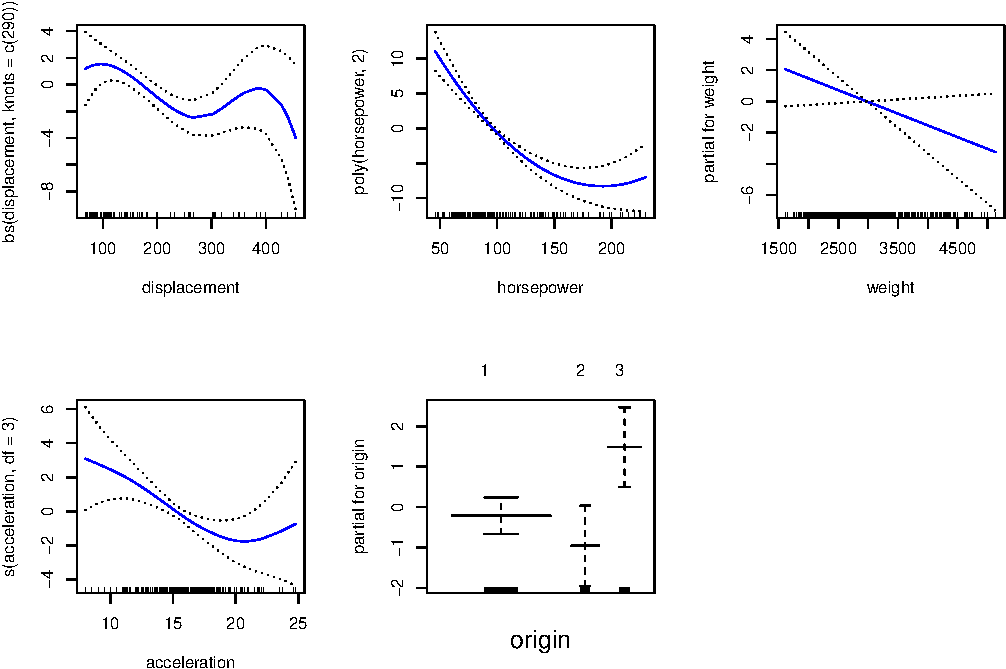
\includegraphics{RecEx11-sol_files/figure-latex/unnamed-chunk-7-1.pdf}

\begin{Shaded}
\begin{Highlighting}[]
\NormalTok{model }\OperatorTok\StringTok{ }\KeywordTok{evaluate}\NormalTok{(x_test, y_test)}
\end{Highlighting}
\end{Shaded}

\begin{verbatim}
## $loss
## [1] 0.2619604
## 
## $accuracy
## [1] 0.9259
\end{verbatim}

Number of parameters

\begin{Shaded}
\begin{Highlighting}[]
\KeywordTok{str}\NormalTok{(model)}
\end{Highlighting}
\end{Shaded}

\begin{verbatim}
## Model
## Model: "sequential"
## ________________________________________________________________________________
## Layer (type)                        Output Shape                    Param #     
## ================================================================================
## dense (Dense)                       (None, 8)                       6280        
## ________________________________________________________________________________
## dense_1 (Dense)                     (None, 8)                       72          
## ________________________________________________________________________________
## dense_2 (Dense)                     (None, 10)                      90          
## ================================================================================
## Total params: 6,442
## Trainable params: 6,442
## Non-trainable params: 0
## ________________________________________________________________________________
\end{verbatim}

\hypertarget{b-3}{%
\subsubsection{b)}\label{b-3}}

\begin{Shaded}
\begin{Highlighting}[]
\NormalTok{model =}\StringTok{ }\KeywordTok{keras_model_sequential}\NormalTok{() }\OperatorTok\StringTok{ }\KeywordTok{layer_dense}\NormalTok{(}\DataTypeTok{units =} \DecValTok{128}\NormalTok{, }\DataTypeTok{activation =} \StringTok{"relu"}\NormalTok{, }
    \DataTypeTok{input_shape =} \KeywordTok{c}\NormalTok{(}\DecValTok{28} \OperatorTok{*}\StringTok{ }\DecValTok{28}\NormalTok{)) }\OperatorTok\StringTok{ }\KeywordTok{layer_dense}\NormalTok{(}\DataTypeTok{units =} \DecValTok{128}\NormalTok{, }\DataTypeTok{activation =} \StringTok{"relu"}\NormalTok{) }\OperatorTok\StringTok{ }
\StringTok{    }\KeywordTok{layer_dense}\NormalTok{(}\DataTypeTok{units =} \DecValTok{10}\NormalTok{, }\DataTypeTok{activation =} \StringTok{"softmax"}\NormalTok{)}

\NormalTok{model }\OperatorTok\StringTok{ }\KeywordTok{compile}\NormalTok{(}\DataTypeTok{optimizer =} \StringTok{"rmsprop"}\NormalTok{, }\DataTypeTok{loss =} \StringTok{"categorical_crossentropy"}\NormalTok{, }
    \DataTypeTok{metrics =} \KeywordTok{c}\NormalTok{(}\StringTok{"accuracy"}\NormalTok{))}

\NormalTok{history =}\StringTok{ }\NormalTok{model }\OperatorTok\StringTok{ }\KeywordTok{fit}\NormalTok{(x_train, y_train, }\DataTypeTok{epochs =} \DecValTok{20}\NormalTok{, }\DataTypeTok{batch_size =} \DecValTok{128}\NormalTok{, }
    \DataTypeTok{validation_split =} \FloatTok{0.2}\NormalTok{)}

\KeywordTok{str}\NormalTok{(history)}
\end{Highlighting}
\end{Shaded}

\begin{verbatim}
## List of 2
##  $ params :List of 7
##   ..$ metrics      : chr [1:4] "loss" "accuracy" "val_loss" "val_accuracy"
##   ..$ epochs       : int 20
##   ..$ steps        : num 375
##   ..$ do_validation: logi TRUE
##   ..$ samples      : int 48000
##   ..$ batch_size   : int 128
##   ..$ verbose      : int 0
##  $ metrics:List of 4
##   ..$ loss        : num [1:20] 0.3347 0.1414 0.0962 0.0727 0.0573 ...
##   ..$ val_accuracy: num [1:20] 0.951 0.961 0.969 0.973 0.973 ...
##   ..$ val_loss    : num [1:20] 0.1742 0.1249 0.1063 0.0908 0.0989 ...
##   ..$ accuracy    : num [1:20] 0.904 0.957 0.971 0.978 0.983 ...
##  - attr(*, "class")= chr "keras_training_history"
\end{verbatim}

\begin{Shaded}
\begin{Highlighting}[]
\KeywordTok{plot}\NormalTok{(history)}
\end{Highlighting}
\end{Shaded}

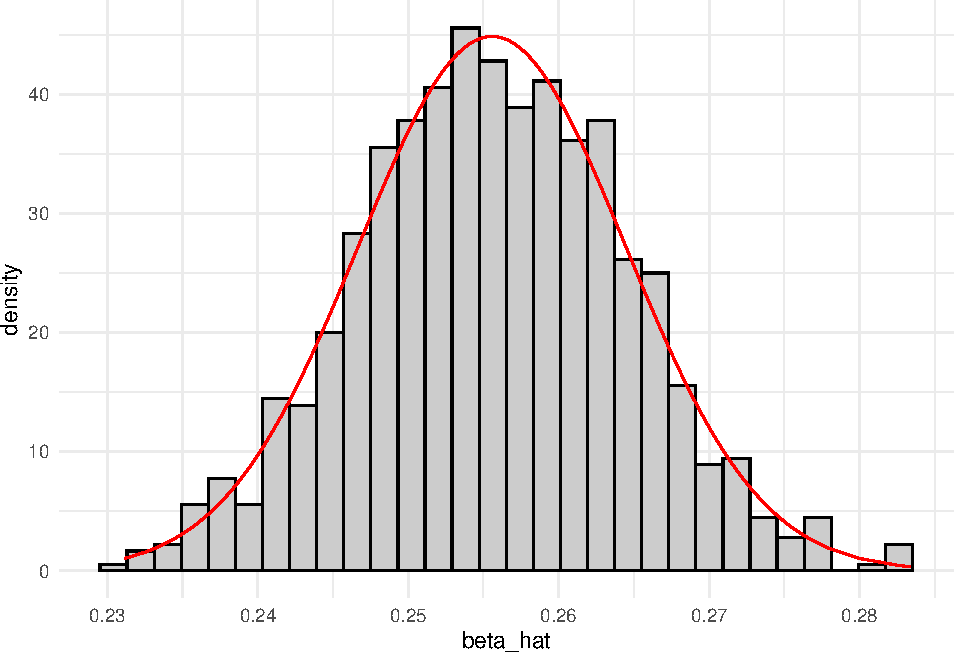
\includegraphics{RecEx11-sol_files/figure-latex/unnamed-chunk-10-1.pdf}

\begin{Shaded}
\begin{Highlighting}[]
\NormalTok{model }\OperatorTok\StringTok{ }\KeywordTok{evaluate}\NormalTok{(x_test, y_test)}
\end{Highlighting}
\end{Shaded}

\begin{verbatim}
## $loss
## [1] 0.1379396
## 
## $accuracy
## [1] 0.9776
\end{verbatim}

We see that the validation loss reach its minimum after 5-10 epochs and
raises again afterwards. This larger network thus begins overfitting
after the first few epochs.

\hypertarget{c-2}{%
\subsubsection{c)}\label{c-2}}

\begin{Shaded}
\begin{Highlighting}[]
\NormalTok{model =}\StringTok{ }\KeywordTok{keras_model_sequential}\NormalTok{() }\OperatorTok\StringTok{ }\KeywordTok{layer_dense}\NormalTok{(}\DataTypeTok{units =} \DecValTok{128}\NormalTok{, }\DataTypeTok{activation =} \StringTok{"relu"}\NormalTok{, }
    \DataTypeTok{input_shape =} \KeywordTok{c}\NormalTok{(}\DecValTok{28} \OperatorTok{*}\StringTok{ }\DecValTok{28}\NormalTok{)) }\OperatorTok\StringTok{ }\KeywordTok{layer_dropout}\NormalTok{(}\DataTypeTok{rate =} \FloatTok{0.4}\NormalTok{) }\OperatorTok\StringTok{ }\KeywordTok{layer_dense}\NormalTok{(}\DataTypeTok{units =} \DecValTok{128}\NormalTok{, }
    \DataTypeTok{activation =} \StringTok{"relu"}\NormalTok{) }\OperatorTok\StringTok{ }\KeywordTok{layer_dropout}\NormalTok{(}\DataTypeTok{rate =} \FloatTok{0.3}\NormalTok{) }\OperatorTok\StringTok{ }\KeywordTok{layer_dense}\NormalTok{(}\DataTypeTok{units =} \DecValTok{10}\NormalTok{, }
    \DataTypeTok{activation =} \StringTok{"softmax"}\NormalTok{)}

\NormalTok{model }\OperatorTok\StringTok{ }\KeywordTok{compile}\NormalTok{(}\DataTypeTok{optimizer =} \StringTok{"rmsprop"}\NormalTok{, }\DataTypeTok{loss =} \StringTok{"categorical_crossentropy"}\NormalTok{, }
    \DataTypeTok{metrics =} \KeywordTok{c}\NormalTok{(}\StringTok{"accuracy"}\NormalTok{))}

\NormalTok{history =}\StringTok{ }\NormalTok{model }\OperatorTok\StringTok{ }\KeywordTok{fit}\NormalTok{(x_train, y_train, }\DataTypeTok{epochs =} \DecValTok{20}\NormalTok{, }\DataTypeTok{batch_size =} \DecValTok{128}\NormalTok{, }
    \DataTypeTok{validation_split =} \FloatTok{0.2}\NormalTok{)}

\KeywordTok{str}\NormalTok{(history)}
\end{Highlighting}
\end{Shaded}

\begin{verbatim}
## List of 2
##  $ params :List of 7
##   ..$ metrics      : chr [1:4] "loss" "accuracy" "val_loss" "val_accuracy"
##   ..$ epochs       : int 20
##   ..$ steps        : num 375
##   ..$ do_validation: logi TRUE
##   ..$ samples      : int 48000
##   ..$ batch_size   : int 128
##   ..$ verbose      : int 0
##  $ metrics:List of 4
##   ..$ loss        : num [1:20] 0.522 0.256 0.205 0.177 0.161 ...
##   ..$ val_accuracy: num [1:20] 0.941 0.956 0.964 0.966 0.968 ...
##   ..$ val_loss    : num [1:20] 0.196 0.152 0.122 0.12 0.109 ...
##   ..$ accuracy    : num [1:20] 0.838 0.925 0.939 0.948 0.953 ...
##  - attr(*, "class")= chr "keras_training_history"
\end{verbatim}

\begin{Shaded}
\begin{Highlighting}[]
\KeywordTok{plot}\NormalTok{(history)}
\end{Highlighting}
\end{Shaded}

\includegraphics{RecEx11-sol_files/figure-latex/unnamed-chunk-12-1.pdf}

\begin{Shaded}
\begin{Highlighting}[]
\NormalTok{model }\OperatorTok\StringTok{ }\KeywordTok{evaluate}\NormalTok{(x_test, y_test)}
\end{Highlighting}
\end{Shaded}

\begin{verbatim}
## $loss
## [1] 0.01524244
## 
## $accuracy
## [1] 0.9955599
\end{verbatim}

Here the validation curve looks better and we might increase the number
of epochs.

\begin{Shaded}
\begin{Highlighting}[]
\NormalTok{model =}\StringTok{ }\KeywordTok{keras_model_sequential}\NormalTok{() }\OperatorTok\StringTok{ }\KeywordTok{layer_dense}\NormalTok{(}\DataTypeTok{units =} \DecValTok{128}\NormalTok{, }\DataTypeTok{activation =} \StringTok{"relu"}\NormalTok{, }
    \DataTypeTok{input_shape =} \KeywordTok{c}\NormalTok{(}\DecValTok{28} \OperatorTok{*}\StringTok{ }\DecValTok{28}\NormalTok{), }\DataTypeTok{kernel_regularizer =} \KeywordTok{regularizer_l2}\NormalTok{(}\DataTypeTok{l =} \FloatTok{0.001}\NormalTok{)) }\OperatorTok\StringTok{ }
\StringTok{    }\KeywordTok{layer_dense}\NormalTok{(}\DataTypeTok{units =} \DecValTok{128}\NormalTok{, }\DataTypeTok{activation =} \StringTok{"relu"}\NormalTok{, }\DataTypeTok{kernel_regularizer =} \KeywordTok{regularizer_l2}\NormalTok{(}\DataTypeTok{l =} \FloatTok{0.001}\NormalTok{)) }\OperatorTok\StringTok{ }
\StringTok{    }\KeywordTok{layer_dense}\NormalTok{(}\DataTypeTok{units =} \DecValTok{10}\NormalTok{, }\DataTypeTok{activation =} \StringTok{"softmax"}\NormalTok{)}

\NormalTok{model }\OperatorTok\StringTok{ }\KeywordTok{compile}\NormalTok{(}\DataTypeTok{optimizer =} \StringTok{"rmsprop"}\NormalTok{, }\DataTypeTok{loss =} \StringTok{"categorical_crossentropy"}\NormalTok{, }
    \DataTypeTok{metrics =} \KeywordTok{c}\NormalTok{(}\StringTok{"accuracy"}\NormalTok{))}

\NormalTok{history =}\StringTok{ }\NormalTok{model }\OperatorTok\StringTok{ }\KeywordTok{fit}\NormalTok{(x_train, y_train, }\DataTypeTok{epochs =} \DecValTok{20}\NormalTok{, }\DataTypeTok{batch_size =} \DecValTok{128}\NormalTok{, }
    \DataTypeTok{validation_split =} \FloatTok{0.2}\NormalTok{)}

\KeywordTok{str}\NormalTok{(history)}
\end{Highlighting}
\end{Shaded}

\begin{verbatim}
## List of 2
##  $ params :List of 7
##   ..$ metrics      : chr [1:4] "loss" "accuracy" "val_loss" "val_accuracy"
##   ..$ epochs       : int 20
##   ..$ steps        : num 375
##   ..$ do_validation: logi TRUE
##   ..$ samples      : int 48000
##   ..$ batch_size   : int 128
##   ..$ verbose      : int 0
##  $ metrics:List of 4
##   ..$ loss        : num [1:20] 0.579 0.336 0.263 0.222 0.198 ...
##   ..$ val_accuracy: num [1:20] 0.944 0.958 0.965 0.968 0.97 ...
##   ..$ val_loss    : num [1:20] 0.385 0.292 0.244 0.215 0.199 ...
##   ..$ accuracy    : num [1:20] 0.898 0.95 0.961 0.968 0.971 ...
##  - attr(*, "class")= chr "keras_training_history"
\end{verbatim}

\begin{Shaded}
\begin{Highlighting}[]
\KeywordTok{plot}\NormalTok{(history)}
\end{Highlighting}
\end{Shaded}

\includegraphics{RecEx11-sol_files/figure-latex/unnamed-chunk-14-1.pdf}

\begin{Shaded}
\begin{Highlighting}[]
\NormalTok{model }\OperatorTok\StringTok{ }\KeywordTok{evaluate}\NormalTok{(x_test, y_test)}
\end{Highlighting}
\end{Shaded}

\begin{verbatim}
## $loss
## [1] 0.03626197
## 
## $accuracy
## [1] 0.9938795
\end{verbatim}

\end{document}
